%!TEX encoding = UTF8
%!TEX root =notes.tex

\chapter{Croissance linéaire}

	\section{Suites arithmétiques}

	\subsection{Définitions}

	\dfn{Suite}{
		Une suite $u$ est une fonction qui à tout entier naturel $n \in \N$ associe un réel
			\[ u(n) \in \R. \]
		Le \emph{terme initial} de la suite est donné par $u(0)$, et son terme de \emph{rang} $n$ est $u(n)$.
	}{}
	
	\ex{}{
		Les fonctions suivantes sont des suites données par leur rang $n$ : on connait donc leur valeur pour tout les entiers naturels.
		\begin{multicols}{2}
		\begin{enumerate}
			\item $u(n) = n+1$
			\item $v(n) = 15 + n$
			\item $\xi(n) = 3n + 1$
			\item $a(n) = n^2$
		\end{enumerate}
		\end{multicols}
		Une suite n'a pas forcément de formule générale pour tout $n$, c'est une simplement \emph{suite} de nombres réels.
	}{}
	
	%Les exercices étudiés en cours nous ont menés à considérer les suites ayant une structure particulière : les suites obtenue par ajouts successifs d'une même constante.
	
	\dfn{Suite arithmétique}{
		On dit d'une suite $u$ qu'elle est arithmétique dès qu'elle vérifie, pour tout $n\in\N$,
			\begin{align}\label{eq:1}
				u(n+1) - u(n) = r,
			\end{align}
		où $r \in \R$ est un réel fixé qui ne dépend pas de $n$.
		
		On appelle $r$ la \emph{raison} de la suite.
	}{}
	
	\nt{
		L'équation \eqref{eq:1} peut se réécrire comme
			\begin{align}\label{eq:2}
				u(n+1) = u(n) + r
			\end{align}
		Avec des mots, on lira alors \og le terme $n+1$ est égal au terme $n$ plus $r$ \fg, et ceci toujours pour tout $n\in\N$.
	}
	
	\nt{
		Pour vérifier qu'une suite est arithmétique et pour connaître sa raison, on préférera l'écriture \eqref{eq:1}.
		L'écriture \eqref{eq:2} est utile pour calculer les terms successifs d'une suite.
	}
	
	
	\ex{}{
		Soit $u$ la suite de terme initial $u(0) = -2$ et de raison $3$.
		
		L'équation \eqref{eq:2} spécialisée en $n=0 \in \N$ donne
			\[ u(1) = u(0) + 3 = -2 + 3 = 1. \]
		Puis, en $n=1 \in \N$, on trouve
			\[ u(2) = u(1) + 3 = 1 + 3 = 4. \]
		Etc... pour avoir
			\begin{align*}
				u(3) &= 7 & u(4) &= 10 & u(5) &= 13 & \cdots
			\end{align*}
		On conjecture que le terme de rang $n\in\N$ s'écrit alors
				\[ u(n) = -2 + 3n. \]
		Le théorème \ref{thm:lili} démontrera cette conjecture.
	}{}
	
	\exe{}{
		Soit $u$ une suite arithmétique de raison $7$ et de terme de rang $61$ donné par
			\[ u(61) = -15.\]
		Calculer $u(63)$.	
	}{}
	
	\ex{}{
		La suite donnée, pour tout $n\in\N$, par
			\[ u(n) = 3n - 2 \]
		est arithmétique.
		En effet, on vérifie que, pour tout $n\in \N$,
			\[ u(n+1) - u(n) = 3(n+1) - 2 - (3n - 2) = 3n + 3 - 2 - 3n + 2 = 3.\]
		Elle est donc arithmétique de raison $3$.
	}{}
	
	\exe{}{
		La suite donnée, pour tout $n\in\N$, par
			\[ \zeta(n) = - n\sqrt{2} + 2\pi \]
		est-elle arithmétique ?
		
		Si oui, donner sa raison et son terme initial. Sinon, justifier.
	}{}
	
	\exe{}{
		Soit $\beta$ la suite donnée, pour tout $n\in\N$, par
			\[ \beta(n) = 3n^3 + \tau, \]
		où $\tau$ est une constante réelle située dans l'intervalle $]1 ; 2[$.
		
		La suite $\beta$ est-elle arithmétique ?		
		Si oui, donner sa raison et son terme initial. Sinon, justifier.
	}{}
	
	\nt{
		L'équation \eqref{eq:1} peut être utilisée pour déduire les variations d'une suite arithmétique selon le signe de sa raison.
		Par exemple, si $r > 0$, alors
			\[ u(n+1) > u(n) \]
		pour tout $n\in\N$
		
		On lira \og le terme $n+1$ est strictement supérieur au terme $n$, pour tout entier naturel $n$ \fg.
		De fait, $u$ est donc croissante.
	}
	
	\dfn{}{
		Pour $u$ une suite arithmétique de raison $r\in\R$. On dit que
		\[\begin{cases*} 
			& $u$ est \emph{croissante} dès que $r > 0$, \\
			& $u$ est \emph{constante} dès que $r=0$, et \\
			& $u$ est \emph{décroissante} dès que $r < 0$.
		\end{cases*}\]
	}
	
	\exe{}{
		Les suites suivantes sont-elles croissantes, décroissantes, ou constantes ? 
		
		\begin{enumerate}
			\item La suite de raison 3 et de terme initial -8.
			\item La suite de raison 0 et de terme initial 3.
			\item La suite $f$ donnée par $f(n) = 3n - 1$ pour tout $n\in\N$.
			\item La suite $g$ donnée par $g(n) = \dfrac1{-4}n + 0$ pour tout $n\in\N$.
		\end{enumerate}
	
	}{}
	
	\subsection{Théorèmes fondamentaux}
	
	\thm{}{
		Soit une suite arithmétique $u$ de terme initial $u(0)\in\R$ et de raison $r \in \R$.
		
		Alors, le terme de rang $n\in\N$ de $u$ est égal à
			\[ u(n) = r \cdot n + u(0). \]	
	}{thm:lili}
	
	\pf{Preuve par itération}{
		On utilise l'équation \eqref{eq:2} en la spécialisant en $n=1, 2, 3, \dots$ jusqu'au terme de rang $n$.
			\begin{align*}
				u(1) &= u(0) + r \\
				u(2) &= u(1) + r = u(0) + r + r = u(0) + 2r \\
				u(3) &= u(2) + r = u(0) + 2r + r = u(3) + 3r \\
				 &\vdots \\
				u(n) &= u(n-1) + r = \dots = u(0) + (n-1)r + r = u(0) + r \cdot n
			\end{align*}	
	}
	\pf{Preuve par somme téléscopique}{
		On utilise l'équation \eqref{eq:1} en la spécialisant de la même façon.
			\begin{align*}
				u(1) - u(0) &= r \\
				u(2) - u(1) &= r \\
				u(3) - u(2) &= r \\
				&\vdots \\
				u(n) - u(n-1) &= r
			\end{align*}
		En ajoutant chaque terme de la gauche un à un, on obtient une somme appelé \emph{téléscopique}.
		On a d'abord $u(1) - u(0)$, puis
			\[ \left(u(1) - u(0)\right) + \left(u(2) - u(1)\right) = u(2) - u(0), \]
		puis
			\[ \left(u(1) - u(0)\right) + \left(u(2) - u(1)\right) + \left(u(3) - u(2)\right) = u(3) - u(0), \]
		etc...
		Or, chaque différence est égale à $r$. La $n$-ième somme donnera donc
			\[ r + r + \dots + r = u(n) - u(0) = r \cdot n, \]
		d'où le résultat.
	}
	
	\ex{}{
		Une suite $\chi$ de terme initial $-12$ et de raison $\pi$ est donnée, pour tout $n\in\N$, par
			\[ \chi(n) = \pi n - 12. \]
	}{}
	
	\nt{
		Il est souvent fastidieux (et en fait redondant) de démontrer qu'une suite est bien arithmétique à l'aide de l'équation \eqref{eq:1} à vérifier pour tous les entiers naturels.
		
		Le théorème \ref{thm:faustine} suivant donne la réciproque du théorème \ref{thm:lili} et permet de conclure du caractère arithmétique ou non d'une suite en voyant son expression au rang $n\in\N$.
	}
	
	\thm{}{
		Soit $u$ une suite donnée par, pour tout $n\in\N$,
			\[ u(n) = r \cdot n + b. \]
		Alors $u$ est arithmétique de raison $r$ et de terme initial $u(0) = b$.
	
	}{thm:faustine}
	
	\pf{Démonstration}{
		Soit $u$ la suite de l'énoncé.
		Considérons une nouvelle suite $v$ de terme initial $b$ et de raison $r$.
		Alors, par le théorème \ref{thm:lili}, le terme de rang $n$ s'écrit, pour tout $n\in\N$,
			\[ v(n) = r \cdot n + b. \]
		On reconnaît l'expression de $u$, et donc
			\[ v(n) = u(n) \]
		pour tout $n\in\N$.
		Les suites $u$ et $v$ sont égales en tout rang et donc égales comme suites.
		Ainsi $u$ est arithmétique de raison $r$ et de terme initial $b$.
	}
	
	\nt{
		On aurait également pû démontrer le théorème \ref{thm:faustine} en utilisant la définition d'une suite arithmétique donnée en \eqref{eq:1}.
		On calcule alors calmement que, pour tout $n\in\N$,
			\begin{align*}
				u(n + 1) - u(n) &= r(n+1) + b - \left( rn + b \right) \\
							&= rn + r + b - rn -b \\
							&= r,
			\end{align*}
		et que le terme initial est donné par $u(0) = r \times 0 + b = b$
		
		Nous voilà rassurés.
	}

	\subsection{Problèmes de seuil}

	\nt{
		Savoir résoudre les inégalités sur les entiers sert à répondre aux questions du type
			\begin{enumerate}
				\item À partir de quel rang la suite dépasse-t-elle une valeur donnée ?
				\item Quels sont les rangs pour lesquels une suite est inférieure (ou égale) à une autre suite ?
			\end{enumerate}
		La notion de \og dépassement \fg est à comprendre dans les deux sens : on peut cherche à savoir pour quels rangs une suite est supérieure à un certain seuil, ou inférieure.
	}
	
	\exe{}{
		Soient les suites données par, pour tout $n\in\N$,
			\[ u(n) = 3n + 1, \qquad v(n) = -3n + 12.\]
		Pour quels rangs $n\in\N$ l'inégalité suivante est-elle vérifiée ?
			\[ u(n) \leq v(n). \]
		On remarque que le terme initial de $v$ est supérieur à celui de $u$ et donc que la réponse devra au moins contenir le rang $0$.
	}{}
	
	\exe{}{
		Pour $u$ une suite donnée par, pour tout $n\in\N$,
			\[ u(n) = 3918n + 60 000. \]
		À partir de quel rang $N\in\N$ la suite $u$ dépasse-t-elle deux fois sa valeur initiale ?
	}{}
	
	\pf{Solution}{
		On cherche à trouver le premier rang $N\in\N$ tel que
			\[ u(N) \geq 2u(0). \]
		Ceci se substitut en
			\[ 3918N + 60 000 \geq 120 000. \]
		On soustrait la valeur initale des deux côtés, puis on divise par 3918.
		\textbf{Le sens de l'inégalité reste inchangé car $3918$ est positif.}
		D'où
			\[ N \geq \dfrac{60 000}{3918} \approx 15,3. \]
		Le premier $N \in \N$ vérifiant cette inégalité est donc $N=16$.
	}
	
	\exe{}{
		Pour $u$ une suite donnée par, pour tout $n\in\N$,
			\[ u(n) = -43n +450. \]
		À partir de quel rang $N\in\N$ la suite $u$ devient-elle négative ou nulle ?
	}{}
	
	\exe{}{
		Donner l'ensemble des $n\in\N$ vérifiants l'inégalité suivante.
			\[ -\dfrac47 n + 9 \leq 3. \]
	}{}
	
	\textbf{Attention : multiplier par un nombre strictement négatif change le sens des inégalités.}
	
	\subsection{Lecture graphique}
	
	On peut représenter une suite en deux dimensions en notant, pour chaque rang $n\in\N$, sa valeur dans un graphe.
	
		\ex{}{
		On note les points de la suite $t$ dans le repère ci-après.
		Un point en coordonnées $(n,y)$ signifie que
			\[ t(n) = y. \]
		$t(n)$ est l'ordonnée du point d'abscisse $n$ (sa hauteur dans le graphe).
		
		\begin{center}
		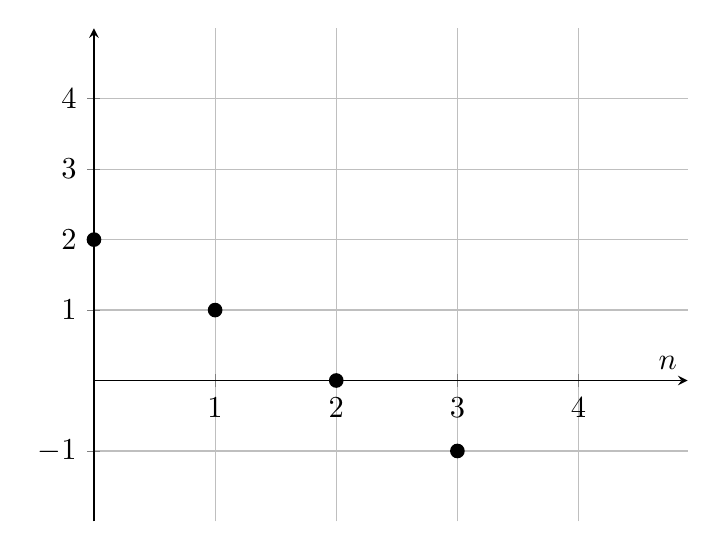
\begin{tikzpicture}[>=stealth, scale=1.1]
			\begin{axis}[xmin = 0, xmax=4.9, xtick={ 0,1,2, 3, 4,5}, ymin=-2, ymax=5, ytick={-1,0,1,2, 3,4}, axis x line=middle, axis y line=middle, axis line style=->, xlabel={$n$}, ylabel={}, grid=both]
				\addplot[black, thick, only marks, mark=*] coordinates {(0,2) (1,1) (2,0) (3,-1)};
			\end{axis}
		\end{tikzpicture}
		\end{center}
		
		On lit alors :
			\begin{align*}
				& t(0) = 2, & t(1) = 1 & t(2) = 0 & t(3) = -1 &
			\end{align*}
		En \emph{sachant} que $t$ est arithmétique, on peut lire sa raison et son terme initial et déduire que $t(n) = 2 - n$ pour tout $n\in\N$.
		
		Si on ne sait pas que $t$ est arithmétique, on ne peut pas le déduire des informations données.
	}{}
	
	\exe{}{
		Nommer et donner le terme de rang $n \in \N$ des suites $\star$, $\bullet$, et $\square$ suivantes données graphiquement.
		\begin{center}
		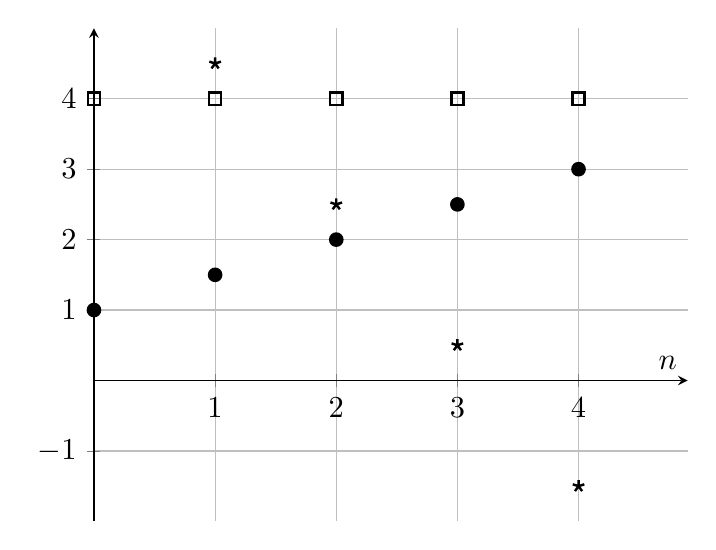
\begin{tikzpicture}[>=stealth, scale=1.1]
			\begin{axis}[xmin = 0, xmax=4.9, xtick={ 0,1,2, 3, 4,5}, ymin=-2, ymax=5, ytick={-1,0,1,2, 3,4}, axis x line=middle, axis y line=middle, axis line style=->, xlabel={$n$}, ylabel={}, grid=both]
				\addplot[black, thick, only marks, mark=*] coordinates {(0,1) (1,1.5) (2,2) (3,2.5) (4,3)};
				
				\addplot[black, thick, only marks, mark=star] coordinates {(1, 4.5) (2,2.5) (3,0.5) (4,-1.5)};
				
				\addplot[black, thick, only marks, mark=square] coordinates {(0,4) (1,4) (2,4) (3,4) (4,4)};
			\end{axis}
		\end{tikzpicture}
		\end{center}
	}{ex:graph-1}
	
	
	\str{
		En ne connaissant pas le terme initial d'une suite, on peut quand même le déduire si on a au moins deux points à disposition.
		C'est le cas de la suite $\star$ de l'exercice \ref{ex:graph-1}. 
		En effet, sa raison est $-2$ et sa valeur en $1$ est $\star(1) = 4.5$.
		
		Le théorème \ref{thm:lili} s'applique toujours, même en posant $P$ sa valeur initiale, inconnue pour l'instant.
		On a alors
			\[ \star(n) = -2n + P, \]
		valable pour tout $n\in\N$, et donc en particulier en $n=1$.
		Ceci implie l'identité suivante, qu'on résoud pour $P$.
			\[ -2 + P = \star(1) = 4.5, \]
		d'où $P = 6.5$.
	}
	
	\nt{
		Dans l'exemple de la suite $\star$ de l'exercice \ref{ex:graph-1}, il est également possible de revenir en arrière en utilisant l'équation \eqref{eq:2}.
		Il faut faire attention à soustraire la raison : on a, pour tout $n\in\R$ et en notant $r$ la raison d'une suite arithmétique $u$, 
			\[ u(n) = u(n+1) - r. \]
		Ici, $\star(0) = \star(1) - (-2) = 4.5 + 2 = 6.5$.
		
		On remerciera les mathématiques de nous donner le même résultat que ci-dessus.
	}
	
	\nt{
		Remarquons qu'une suite arithmétique suit la trace d'une droite. On comparera les définitions
			\begin{align*} & f(x) = ax + b & \text{et} && u(n) = rn + b. & \end{align*}
		
		Il n'est donc pas surprenant qu'il suffise de deux valeurs (distinctes) d'une suite arithmétique pour connaître sa raison et son terme initial, et donc son expression générale.
		En effet, il suffit de deux points d'une droite pour la connaître complètement.	
	}
	
		
	\exe{}{
		Nommer et donner le terme de rang $n \in \N$ des suites $\star$, $\bullet$, et $\square$ suivantes données graphiquement.
		\begin{center}
		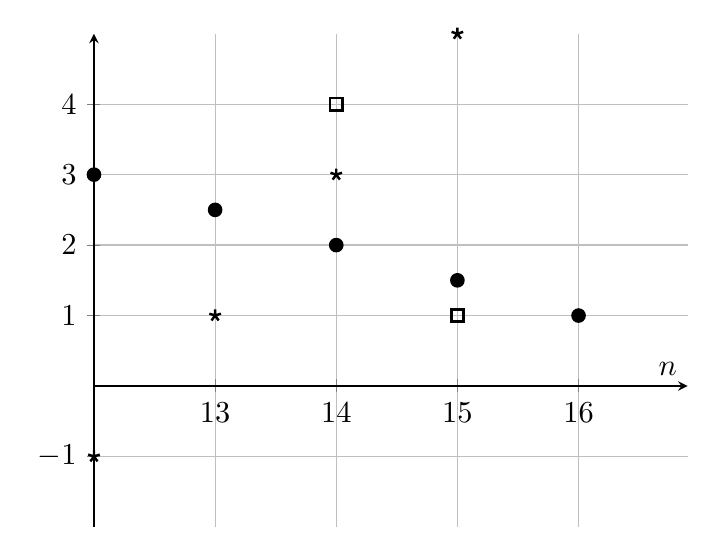
\begin{tikzpicture}[>=stealth, scale=1.1]
			\begin{axis}[xmin = 12, xmax=16.9, xtick={ 12,13,14,15, 16}, ymin=-2, ymax=5, ytick={-1,0,1,2, 3,4}, axis x line=middle, axis y line=middle, axis line style=->, xlabel={$n$}, ylabel={}, grid=both]
				\addplot[black, thick, only marks, mark=*] coordinates {(12,3) (13,2.5) (14,2) (15,1.5) (16,1)};
				
				\addplot[black, thick, only marks, mark=star] coordinates {(12,-1) (13,1) (14,3) (15,5)};
				
				\addplot[black, thick, only marks, mark=square] coordinates {(14,4) (15,1)};
			\end{axis}
		\end{tikzpicture}
		\end{center}
		\textbf{Attention : les rangs commencent à $12$ dans le graphe ci-dessus.}
	}{}
	
	
		\exe{}{
		Nommer et donner le terme de rang $n \in \N$ des suites $\star$, $\bullet$, et $\square$ suivantes données graphiquement.
		\begin{center}
		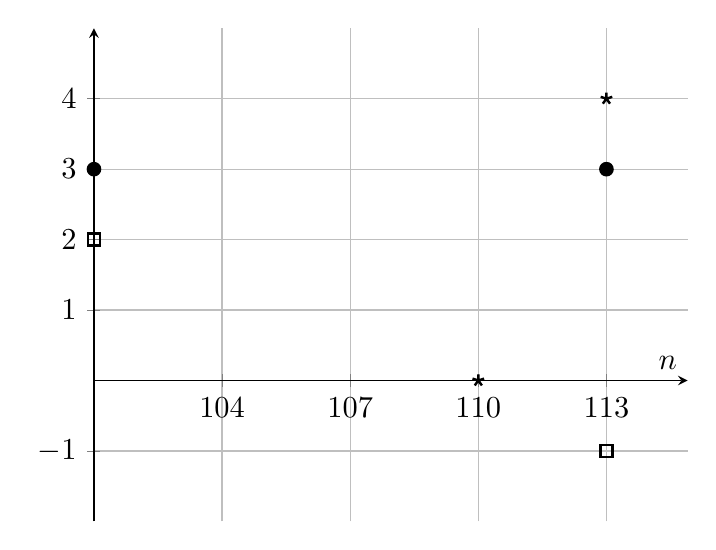
\begin{tikzpicture}[>=stealth, scale=1.1]
			\begin{axis}[xmin = 101, xmax=114.9, xtick={ 101,104,107,110,113}, ymin=-2, ymax=5, ytick={-1,0,1,2, 3,4}, axis x line=middle, axis y line=middle, axis line style=->, xlabel={$n$}, ylabel={}, grid=both]
				\addplot[black, thick, only marks, mark=*] coordinates {(101,3) (113,3)};
				
				\addplot[black, thick, only marks, mark=star] coordinates {(110,0) (113,4)};
				
				\addplot[black, thick, only marks, mark=square] coordinates {(101,2) (113,-1)};
			\end{axis}
		\end{tikzpicture}
		\end{center}
		\textbf{Attention : les rangs commencent à $101$ et vont de $3$ en $3$ dans le graphe ci-dessus. Il manque des points aux suites $\bullet$ et $\square$.}
	}{ex:graph-3}
	
	\pf{Solution pour la suite $\square$}{
		On résoud l'exercice \ref{ex:graph-3} pour la suite $\square$.
		
		Posons d'avance
			\begin{align}\label{eq:sqr-expr} \square(n) = rn + b, \end{align}
		où $r$ est la raison de la suite, et $b$ son terme initial à trouver.
		
		La suite $\square$ étant arithmétique, on a la relation suivante
			\begin{align*}
				\square(113) = \square(101) + 12 r & \iff -1 = 2 + 12r 
			\end{align*}
		qui nous donne $r = -\dfrac14$.
		
		En connaissant le terme de rang $101$, on a donc l'égalité suivante.
			\[ -\dfrac14 \cdot 100 + b = \square(101) = 2, \]
		d'où $b=27$.
	}
	
	\pf{Seconde solution pour la suite $\square$}{
		Par analogie avec les droites, il est possible de résoudre pour $r$ et $b$ de l'expression \eqref{eq:sqr-expr} en posant un système de deux équations à deux inconnues.
		
		Les points $(101;2)$ et $(113;-1)$ se traduisent par les égalités suivantes.		
		\begin{align*}
			\begin{cases*} \square(101) = 2, \\ \square(113) = -1. \end{cases*} 
			&& \iff &&
			\begin{cases*} 101r + b = 2, \\ 113r + b = -1. \end{cases*} 
		\end{align*}
		En soustrayant la première équation à la deuxième, on retrouve la relation
			\[ 12r = -3,\]
		et on conclut de la même manière.
	
	}
	

	